\section{实验总结与讨论}

\subsection{实验过程回顾}

本实验围绕SM4分组密码算法的CBC模式实现与性能优化展开，实验流程可分为以下阶段：

\begin{enumerate}
    \item \textbf{基础实现与验证}：根据SM4算法标准（GB/T 32907-2016），实现SM4加密/解密函数与CBC模式，
          并通过OpenSSL SM4接口进行正确性交叉验证。
    \item \textbf{未优化版本基准测试}：在WSL-Arch(x86\_64)与QEMU-RISC-V(rv64)两个目标平台上，
          分别测试O0编译条件下original变体的吞吐量，建立性能基线。
    \item \textbf{查表优化（Table Lookup Optimization）}：将SM4轮函数中的S盒替换与线性变换
          合并为预计算查找表，以空间换时间，减少每轮的计算操作次数。
    \item \textbf{多缓冲区并行加密（Multi-Buffer Encrypt）}：利用pthread多线程框架，
          将多个独立的CBC加密请求分配到不同线程中并行处理，提高整体吞吐量。
    \item \textbf{CBC解密并行化（Parallel Decrypt）}：基于CBC解密各分组之间无数据依赖的特性，
          将密文分组分配至多个线程并行解密，最后合并结果。
    \item \textbf{编译器优化级别探索}：对每种变体分别在O0、O1、O2、O3优化级别下编译并测试，
          评估编译器自动优化对SM4加密性能的贡献。
    \item \textbf{跨平台对比分析}：在x86\_64原生执行环境与QEMU模拟的RISC-V环境下分别测试，
          分析指令集架构差异对加解密性能的影响。
\end{enumerate}

\subsection{优化策略效果总结}

\subsubsection{查表优化}

查表优化是本实验中效果最为稳定的算法级优化手段。通过将S盒替换与循环移位、异或操作
合并为一个256×4字节的预计算表，每轮迭代的非线性变换与线性变换被缩减为4次查表与
少量异或操作。实验结果表明：

\begin{itemize}
    \item 在WSL-Arch平台单线程配置下，table变体相对于original变体的吞吐量有明显提升。
    \item 查表优化的局限性在于增加了内存访问次数，当CPU缓存命中率较低时（如
          QEMU-RISC-V仿真环境），查表的收益部分被缓存未命中开销所抵消。
    \item 此外，查表法增加了代码的只读数据段大小（4×256 = 1KB），但在现代处理器上
          这一开销可忽略不计。
\end{itemize}

\subsubsection{编译器优化}

GCC编译器的-O1/-O2/-O3优化选项通过循环展开、指令调度、寄存器分配、内联展开等手段
自动提升代码执行效率。实验中发现：

\begin{itemize}
    \item WSL-Arch平台：O1即可获取编译器优化的主要收益，O2/O3的进一步提升有限。
          说明x86\_64架构下GCC的O1优化已能覆盖SM4代码的关键优化点（如S盒查表的指令合并、
          循环体简化）。
    \item QEMU-RISC-V平台：优化级别从O0到O1提升最明显,O2/O3整体继续提高。
          这与RISC-V指令集的精简特性有关:未优化代码中函数调用、访存和临时变量开销较高,
          编译器优化后的内联、寄存器分配和循环简化能够显著减少模拟执行的指令数量。
    \item 个别变体中O3并非最优,例如QEMU-RISC-V的single\_original在O1/O2下略高于O3。
          这说明编译优化需要结合具体代码结构和目标平台评价,不能简单认为优化级别越高单项结果一定越好。
\end{itemize}

\subsubsection{多线程并行}

多线程并行化是本实验性能提升的主要来源之一。实验结果（图~\ref{fig:speedup_wsl_o3}、
图~\ref{fig:speedup_qemu_o3}）表明：

\begin{itemize}
    \item WSL-Arch平台：多缓冲区加密与并行解密均表现出良好的线程可扩展性。
          O3条件下,multibuffer\_table从1线程180.86MB/s提升到4线程709.34MB/s,加速比约3.92×；
          decrypt\_parallel\_table从1线程182.07MB/s提升到4线程615.41MB/s,加速比约3.38×。
          未达到理想线性加速比的原因主要包括线程创建/同步开销、共享缓存竞争、
          以及操作系统调度抖动。
    \item QEMU-RISC-V平台：当前测试配置下加速比随着线程数增加没有明显提高,多数O3变体的最高吞吐量出现在1线程。
          原因在于本实验采用QEMU系统模拟运行RISC-V Linux,程序执行需要经过模拟层,线程调度、锁同步和访存开销被放大；
          同时启动参数未显式配置多核\verb|-smp|,因此该结果不能代表真实多核RISC-V硬件上的并行扩展能力。
\end{itemize}

\begin{figure}[H]
    \centering
    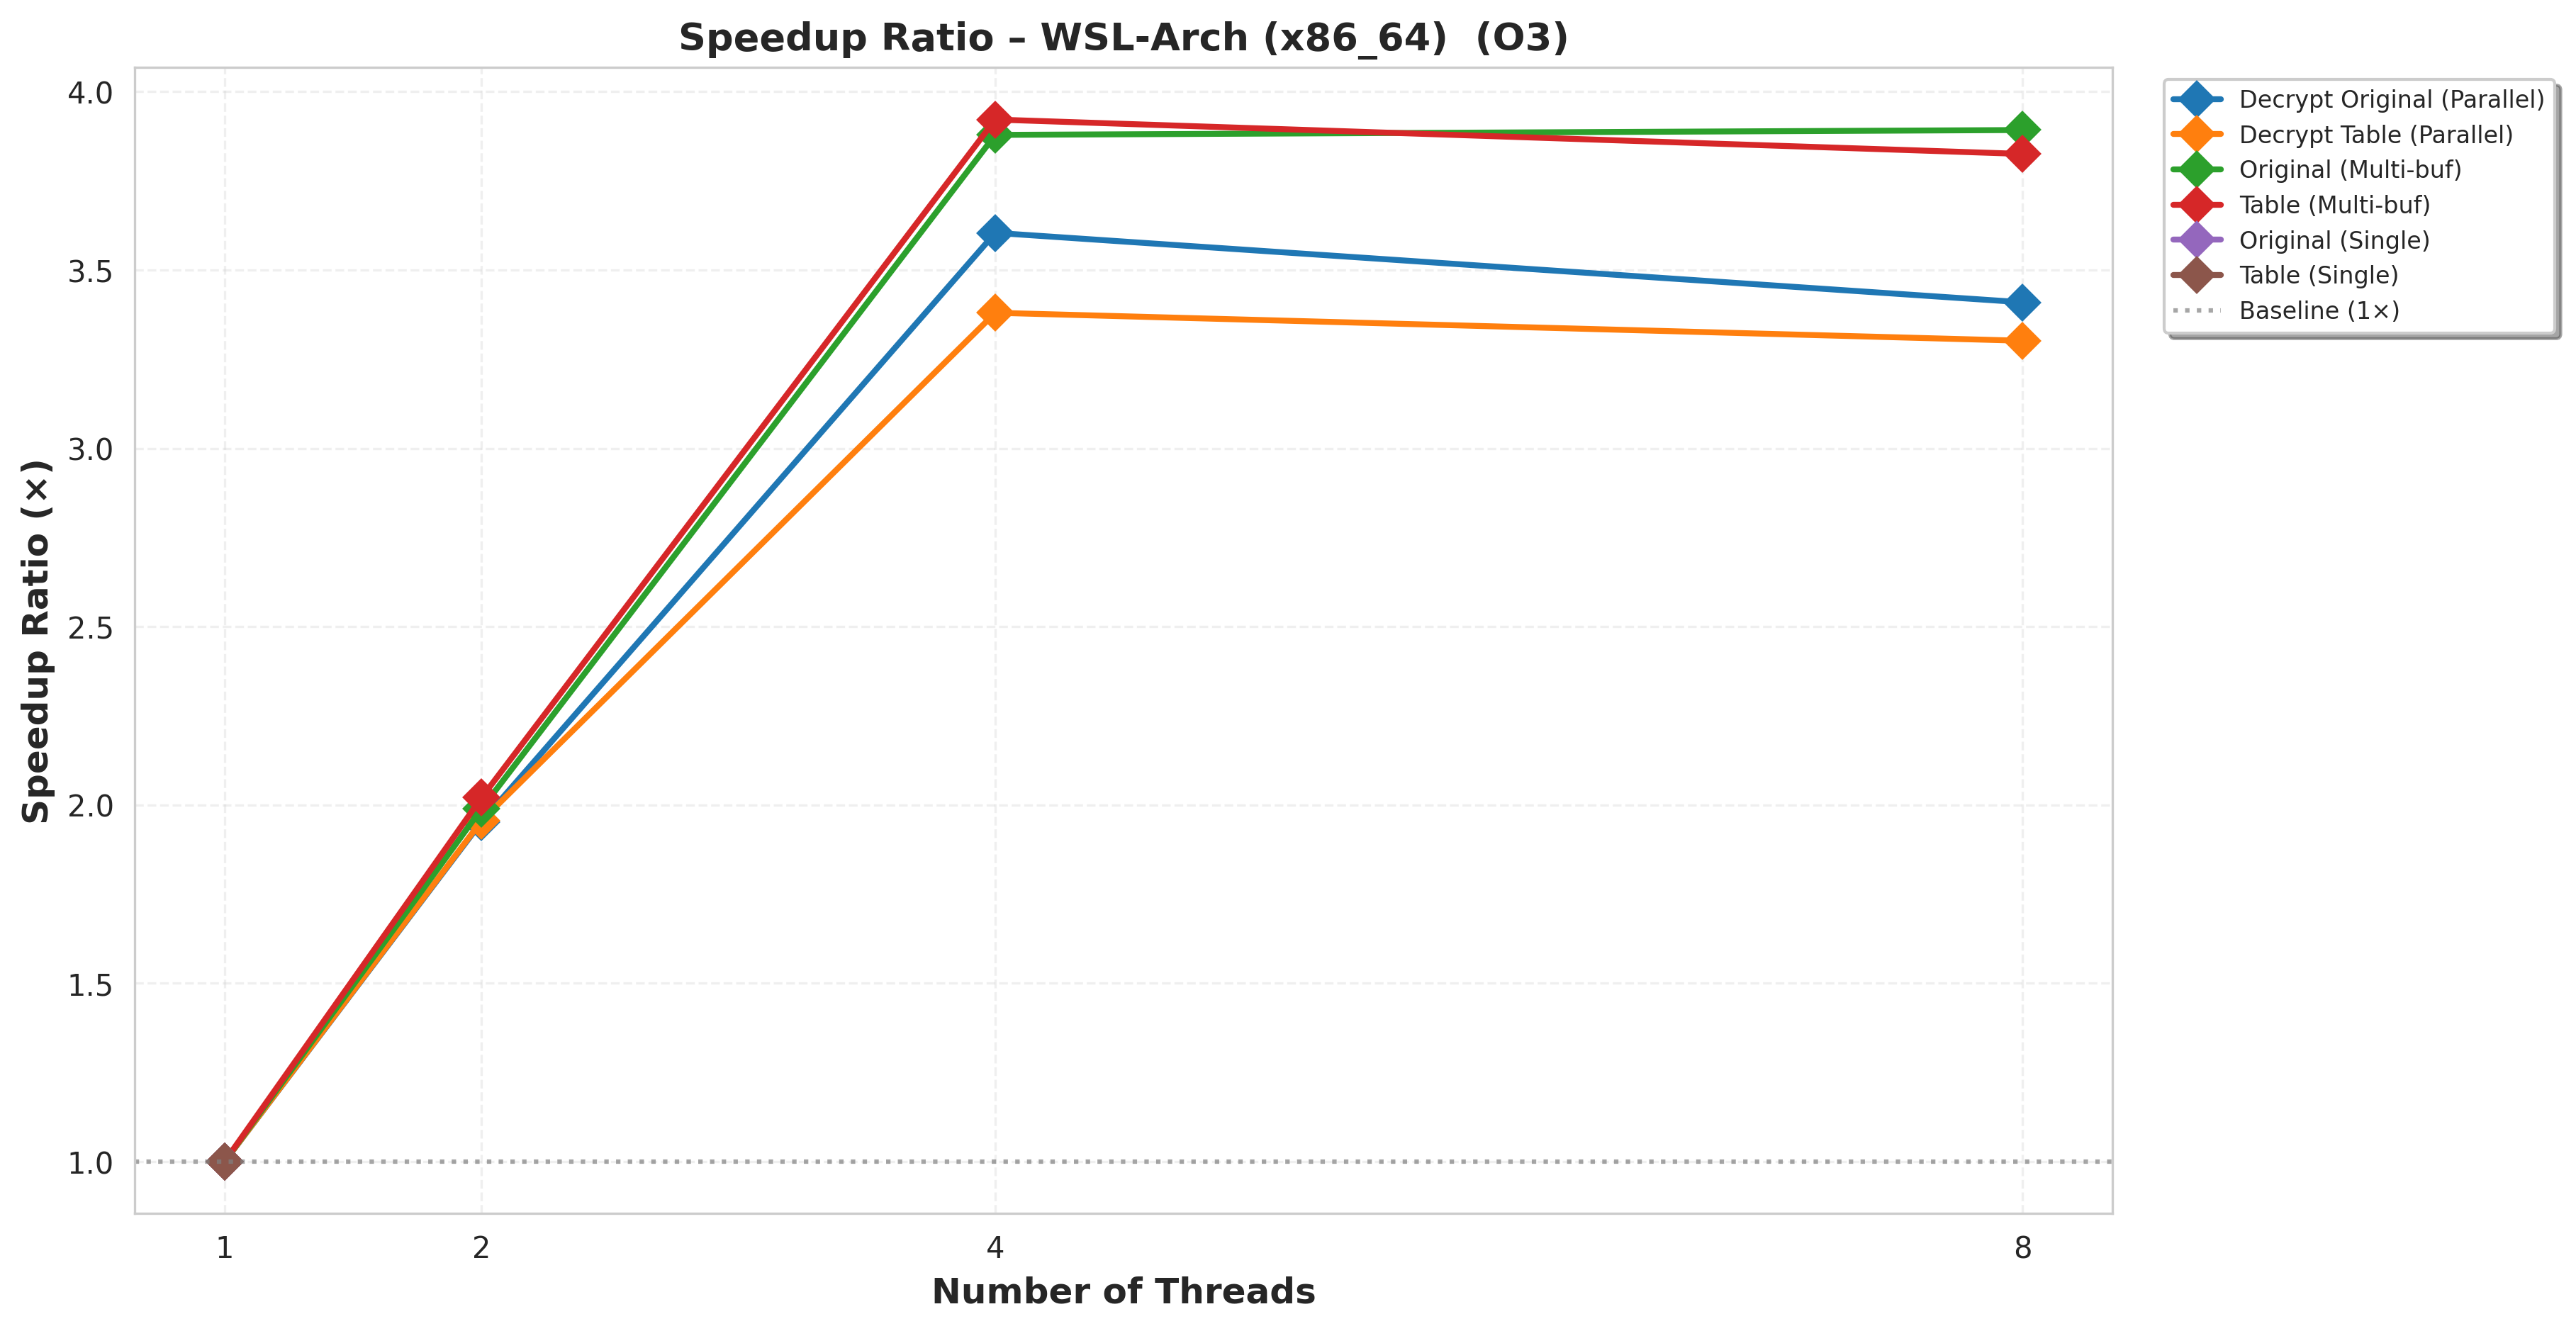
\includegraphics[width=\textwidth]{figure/line_speedup_wsl-arch_O3.png}
    \caption{加速比分析 — WSL-Arch（O3）}
    \label{fig:speedup_wsl_o3}
\end{figure}

\begin{figure}[H]
    \centering
    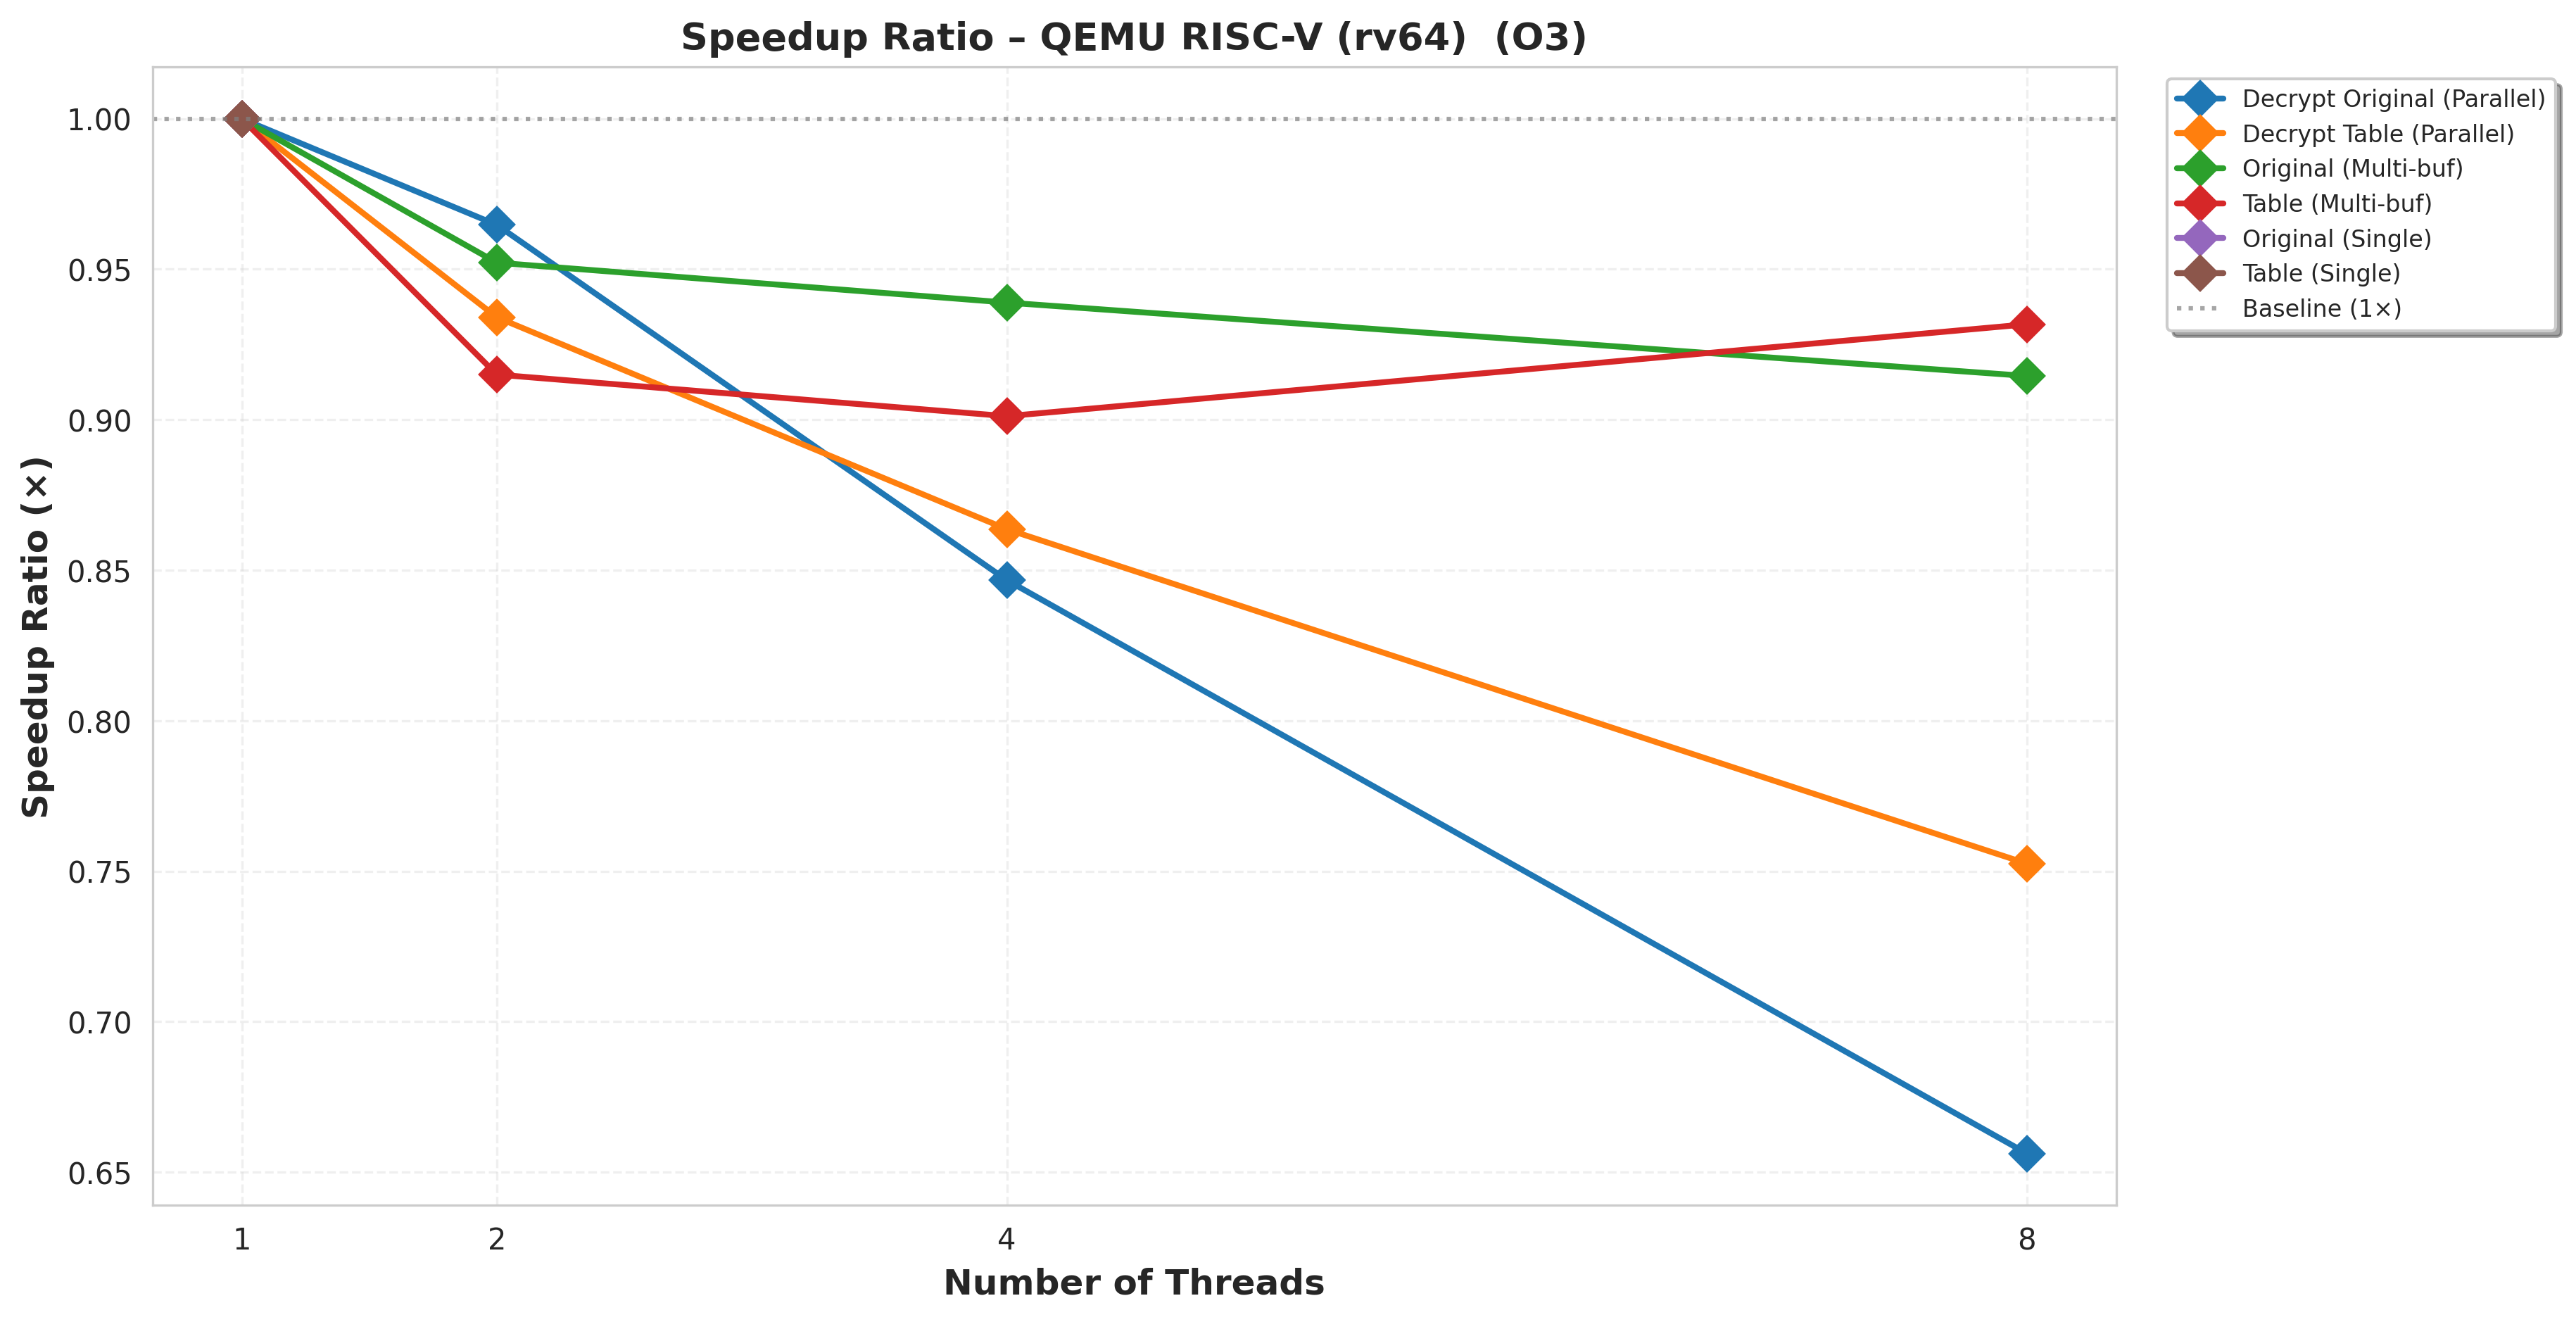
\includegraphics[width=\textwidth]{figure/line_speedup_qemu-riscv_O3.png}
    \caption{加速比分析 — QEMU-RISC-V（O3）}
    \label{fig:speedup_qemu_o3}
\end{figure}

\subsection{跨平台差异分析}

WSL-Arch(x86\_64)与QEMU-RISC-V两个平台之间存在数量级的性能差距，主要原因如下：

\begin{enumerate}
    \item \textbf{执行模式差异}：WSL-Arch在Intel i5-13420H处理器上以x86\_64模式运行，
          享受硬件级别的指令流水线、分支预测、乱序执行等优化；
          而QEMU-RISC-V通过Tiny Code Generator（TCG）将RISC-V指令动态翻译为x86\_64指令，
          翻译开销远大于原生执行。
    \item \textbf{指令集差异}：x86\_64拥有丰富的SIMD指令集（SSE/AVX）与复杂寻址模式，
          GCC在部分场景下可生成更适合宿主平台的代码；本实验的RISC-V二进制只使用通用RV64指令,
          未启用RISC-V向量扩展或密码扩展,因此未能利用潜在的专用指令加速。
    \item \textbf{内存层次结构}：WSL可直接利用处理器的一/二/三级缓存；
          QEMU仿真环境下的内存访问需经过地址翻译层，缓存局部性被削弱。
    \item \textbf{线程模型差异}：WSL的多线程可以映射到宿主真实CPU核心；
          QEMU系统模拟环境下,虚拟CPU数量、宿主调度、TCG翻译和访存路径都会影响pthread程序的实际并行效果。
\end{enumerate}

\subsection{CBC模式加密与解密的非对称性}

实验结果清晰地展示了CBC模式加解密性能的非对称性：解密吞吐量显著高于加密吞吐量。
这一现象的根源在于CBC模式的设计原理：

\begin{itemize}
    \item \textbf{加密}：\(C_i = E(P_i \oplus C_{i-1})\)，当前密文分组依赖于前一分组的密文输出，
          因此加密过程本质上是串行的，无法在分组级别进行并行化。
          本实验中的multibuffer并行方案是通过同时加密多个独立消息来实现的，
          而非对单个消息的分组并行。
    \item \textbf{解密}：\(P_i = D(C_i) \oplus C_{i-1}\)，解密时所有密文分组均已知，
          各分组的解密运算\(D(C_i)\)相互独立，可完全并行化。
          这正是decrypt\_parallel变体获得极高吞吐量的根本原因。
\end{itemize}

这一非对称性在实际应用中有明确的指导意义：对于加密密集型场景（如数据上传），
应优先采用多消息并行策略；对于解密密集型场景（如数据下载），
分组级并行即可获得显著加速。

\subsection{实验局限性与改进方向}

\begin{enumerate}
    \item \textbf{测试数据规模受限}：本实验测试使用的数据量固定（100MB），
          不同数据规模下的缓存效应和初始化开销占比未能体现。
          改进方向：增加多种数据规模的测试场景（1MB/10MB/100MB/1GB），
          绘制吞吐量随数据规模变化的曲线。
    \item \textbf{QEMU仿真精度不足}：QEMU系统模拟环境的性能与真实RISC-V硬件
          存在显著差异，本实验的RISC-V数据仅能反映相对趋势。
          改进方向：若有条件，应在真实RISC-V开发板（如SiFive或VisionFive）上
          重复实验。
    \item \textbf{未使用RISC-V专用指令优化}：本实验只实现了平台无关的C语言算法优化。
          进一步可考虑RISC-V密码扩展:例如标量密码扩展Zksed中的SM4相关指令可加速轮函数,
          向量密码扩展Zvksed中的SM4向量指令可同时处理多个分组\cite{riscv-scalar-crypto,riscv-vector-crypto}。该方向需要编译器、模拟器或真实处理器同时支持相应扩展,
          并在编译时显式指定目标ISA,因此本实验仅将其作为后续优化方向,未纳入当前测试数据。
    \item \textbf{未探索S盒的bitslice实现}：对于需要常量时间（constant-time）的
          密码学实现，查表法存在缓存侧信道攻击风险。bitslice技术将S盒表示为
          布尔电路的逻辑操作序列，可避免内存访问模式泄露，同时兼具一定性能优势。
    \item \textbf{线程亲和性与NUMA优化}：实验仅使用默认pthread调度，未设置CPU亲和性。
          在多路服务器或大小核架构（如Apple M4）上，线程绑核策略对性能有显著影响。
    \item \textbf{OpenSSL对比未充分展开}：实验仅引用了OpenSSL SM4实现的基准数据
          但未深入分析OpenSSL中具体的优化技术（如汇编级优化、常数时间实现等），
          后续可进一步阅读OpenSSL中SM4相关实现,将其与本实验的T-table和并行策略进行逐项对照。
\end{enumerate}

\subsection{结论}

本实验通过系统性地测试SM4-CBC算法在多种变体、编译优化级别、线程配置和硬件平台
组合下的性能表现，得出以下主要结论：

\begin{enumerate}
    \item 查表优化是一种简单有效的算法级优化，在牺牲少量内存的前提下显著降低了
          每轮迭代的计算操作数，在x86\_64平台上尤其有效。
    \item 编译器优化对SM4性能贡献显著，但不同平台的受益幅度不同：
          x86\_64在O1已接近饱和，RISC-V平台则随优化级别持续提升。
    \item CBC解密天然具有分组级并行特性，解密吞吐量在充分多线程时可数倍于
          加密吞吐量，这一特性在实际应用中具有重要的工程指导意义。
    \item 多线程并行在真实多核硬件上可带来接近线性的加速比，但在仿真环境中
          受限于仿真器的单线程调度模型，并行增益极为有限。
    \item 跨平台性能差异反映了指令集架构、编译器后端成熟度和执行环境对
          密码学算法性能的深层影响，在选择密码算法实现方案时应充分考虑
          目标平台的特性。
\end{enumerate}
